\chapter{Benchmark Study}\label{EmChap}
In this chapter, the preparations and the result of the study are described.
With this, the used datasets to determine the performance are defined, and the set of transfer learning classifiers with the corresponding parameters are appointed.\\
Furthermore, the used statistical methods in the study are introduced, and the statistics are shown and discussed.
This study is split up in three main statistics.
The first part is a basic descriptive statistic to give an overview of the general performance of the classifiers.
This is followed by the comparison of classifiers over one dataset and finally over multiple datasets, with this all datasets described in this thesis are tested.\\
The procedure and selection of statistics are mainly adopted from \cite{Chen.2009} and \cite{Long.2015}.
The main reason for this is to guarantee a fair comparison of the \acs{PCVM}, \acs{PCTKVM} and the \acs{TKL} method as wrapper algorithm for the \acs{SVM}.
Note that in this chapter for clarity only the summarised tables are shown. The complete results are shown in appendix\ref{appaB}.

\section{Dataset Description}\label{EmSecDaDes}
The study consists of 18 benchmark datasets.
Three of them are text-based from Reuters-21578\footnote{http://www.daviddlewis.com/resources/testcollections/reuters21578} and the remaining twelve are images from Caltech-256\footnote{http://www.vision.caltech.edu/Image\_Datasets/Caltech256/ } and Office.
Note that the datasets are not extracted from the raw data, but rather used from others with a pre-processing state.
The corresponding articles, which are using this version of datasets are \cite{Gong.} and \cite{Long.2015}.
\\
This 18 sets are well known in the area of domain adaptation and transfer learning and for example used in 
\cite{Long.2015}\cite{Gong.}\cite{Fernando.}\cite{Long.}\cite{Dai.}\cite{Quattoni.} and discussed in \cite{Pan.2010}.\\
A crucial characteristic of the datasets is that the domains for training and testing are different but related.
This relation exists because the train and test classes have the same top category or source.
The classes itself are subcategories or subsets.\cite{JingGao.2008}\\
The relation will be clear in the separate sections for the datasets respectively.

\subsection{Text Dataset}\label{EmSubSecText}
The Reuters-21578 collection appeared on the Reuters news-wire in 1987.
The documents were assembled with categories by personnel from Reuters Ltd. and \ac{CGI}.
Reuters and \acs{CGI} published the documents for research purposes.\cite{DavidD.Lewis.2004}\\
It is a frequently used text collection to evaluate the performance of text categorisation techniques.
The collection is segmented in five top categories and many subcategories.
For testing classifiers, the task is to evaluate on the three big categories \textit{orgs}, \textit{people} and \textit{places}. 
In the last subcategory, all documents about the USA are removed.
This makes the categories nearly even because more than a half of the documents are in the USA subcategory. 
Furthermore, some pre-processing done at the collection.\cite{WenyuanDai.2007}\\
First, all letters are converted to lower case, and the words are stemmed using the Porter stemmer.
This stemmer removes the suffixes form the terms.\cite{Porter.1997} 
Furthermore, stopwords are removed. With the \ac{DF} Thresholding, the numbers of features are cut down.
To apply the \acs{DF} Thresholding the number of documents in which a certain term occurs has to be count.
Each term which is less than a previously set threshold is removed from the feature space.\cite{Yang.1997}
The Threshold parameter is set to three with the goal to speed up the classification process.
Finally, \ac{TFIDF} is applied for feature generation.
The \acs{TFIDF} value is used to train the classifiers.
The \acs{TFIDF} is a measure of how well a term characterizes a document.
It takes the frequency of a term in a document times the inverse document frequency which is the number of occurrences of this term in all documents. \cite[p. 26]{Leskovec.2014}\\
For the domain adaptation purpose, six datasets were generated from Reuters-21578:
\textit{orgs vs places}, \textit{orgs vs people}, \textit{people vs places}, \textit{places vs orgs}, \textit{people vs places} and \textit{places vs people}.
The labels are created by assigning orgs for example as positive class and people as the negative class.
Furthermore, the two labels are split by its subcategories to create the training and test sets.\cite{WenyuanDai.2007}\\
In table \ref{TableSumReuters} the dataset with its features, observations, labels and the corresponding divergences, \acs{KLD} and \ac{MMD}, are shown.
The divergences are defined int Section \ref{TlSubSecKLD}. \\
To get an overview of the distribution and its transfer learning purpose the \textit{orgs vs people} dataset is shown in Figure \ref{FigOrgVsPeoplePlot}.
\begin{table}[]
	\centering
	\resizebox{\textwidth}{!}{%
	\begin{tabular}{c|cccc|c|c}
		Top Category     & \#Examples 1 & \#Examples 2 & \#Features       & \# Labels      & \ac{KLD} & \ac{MMD}\\ \hline
		Orgs vs People   & 1237                  & 1208                  & \multirow{3}{*}{4771} &	\multirow{3}{*}{2} & 0.4570  &   0.0410  \\
		Orgs vs Places   & 1208                  & 1016                  &                       &	 					& 0.7420  &  	0.0455 \\
		People vs Places & 1016                  & 1208                  &                       &						 &  0.6690 &	0.0421   
	\end{tabular}}
	\caption[Overview of key values of Reuters-21578 dataset]{Overview of the key figures of the Reuters-21578 dataset	\label{TableSumReuters}}
\end{table}


\begin{figure}
	\centering
	\begin{subfigure}{.5\textwidth}
		\centering
		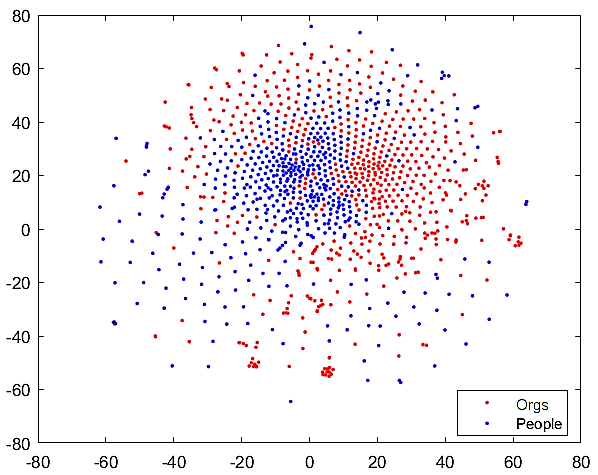
\includegraphics[width=1\linewidth]{figures/Plot_Train_OP_1.png}
		\label{FigOPSub1}
	\end{subfigure}%
	\begin{subfigure}{.5\textwidth}
		\centering
		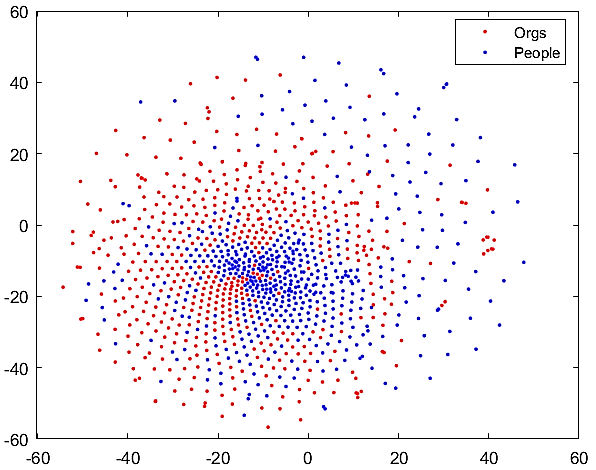
\includegraphics[width=1\linewidth]{figures/Plot_Test_OP_1.png}
		\label{FigOPSub2}
	\end{subfigure}
	\caption[Plot of Orgs vs People Dataset]{The plot of the \textit{Orgs vs People} dataset. One the left hand is the training set, and on the right, the test set is shown. The dimension is reduced with t-SNE to two dimensions. The \acs{KLD} to the original Dataset is 2.233 and 2.464 	\label{FigOrgVsPeoplePlot}}
\end{figure}

\subsection{Image Dataset}\label{EmSubSecIm}
The image dataset has two main Parts. 
The first one which is named \textit{office} in this thesis and is collected and created from \cite{Saenko.2010}.
This contains various images from three different sources which are the different datasets respectively.
One are images taken from the web downloaded from the online merchants \textit{amazon} (Name in Dataset).
Originally 31 categories, which are different types of products, with an average of 90 images are captured.
The objects are typically shown from a canonical viewpoint.\\
A canonical viewpoint is a certain view of an object in a certain rotation, which is considered as 'good' to recognise the object. \cite{Edelman.1991}\\
The second consists of images that are captured with a digital SLR camera (\textit{dslr}).
The conditions should be realistic environments (\textit{office}) and natural lighting.
The resolution of the images is high with low noise.
With that 31 object categories within five different objects are taken.
An object contains on average three images, taken from various viewpoints.
This makes a total of 423 images.\\
The image dataset has two main Parts. 
The first one which is named \textit{office} in this thesis and is collected and created from \cite{Saenko.2010}.
This contains various images from three different sources which are the different datasets respectively.
One are images taken from the web downloaded from the online merchants \textit{amazon} (Name in Dataset).
Originally 31 categories, which are different types of products, with an average of 90 images are captured.
The objects are typically shown from a canonical viewpoint.\\
A canonical viewpoint is a certain view of an object in a certain rotation, which is considered as 'good' to recognise the object. \cite{Edelman.1991}\\
The second consists of images that are captured with a digital SLR camera (\textit{dslr}).
The conditions should be realistic environments (\textit{office}) and natural lighting.
The resolution of the images is high with low noise.
With that 31 object categories within five different objects are taken.
An object contains on average three images, taken from various viewpoints.
This makes a total of 423 images.
The last set of images are from a \textit{webcam}.
Images are taken from this, with a low resolution with a high noise. The purpose of this is to simulate sensors that are similar to robotic sensors.
It has the same 31 categories with five objects per category and a total of 795 images. \\
The second main part of this dataset is from \cite{GregGriffin.}. In comparison with the other image collections, the \textit{Caltech-256} dataset is much larger.
It has an average of 119 images per category in 257 categories with a total of 30607 images.
They are crawled from Google and PicSearch.
Duplicates are deleted. The \ac{SIFT} approach transforms images into scale-invariant coordinates relative to local features which are 'summarised' in key point descriptors.\cite{Lowe.2004}
With this images with over 15 similar \acs{SIFT} descriptors are removed.
The images are sorted in a category itself by the amount of how good this one represents the category.
The Range goes from "Good: A clear example of the visual category" to "Not Applicable: Not an example of the object category.\cite[p.3]{GregGriffin.}\\
To get an overall collection of the four image sets which are considered as domains, categories with the same description are taken.
From the 31 and 256 categories are ten similar categories extracted:
backpack, touring-bike, calculator, head-phones, computer-keyboard, laptop-101, computer-monitor, computer-mouse, coffee-mug and video-projector.
They are the class labels from one to ten. 
With this, a classifier should be trained on the training domain and should be able to classify the test image to the corresponding image category.
The final feature extraction is done with \ac{SURF} and encoded with 800-bin histograms.
Finally, the twelve sets are designed to be trained and tested against each other by the ten labels.\cite{Gong.} \\
The \ac{SURF} Algorithm uses integral images for images convolutions and uses existing detectors and descriptors and reduced the used methods to the essentials. \cite{vanBay.2006} 
In figure \ref{FigExampleImages} are some example images taken from the four datasets of the category computer monitor. 
As in \ref{EmSubSecText}, the some key figures from the dataset are pointed out in table \ref{TableSumImage}.
Note that for clarity, not the twelve datasets are shown, but rather only the 'caltech vs others'.
The remaining sets should be similar.
The last set of images are from a \textit{webcam}.
Images are taken from this, with a low resolution with a high noise. The purpose of this is to simulate sensors that are similar to robotic sensors.
It has the same 31 categories with five objects per category and a total of 795 images. \\
The second main part of this dataset is from \cite{GregGriffin.}. In comparison with the other image collections, the \textit{Caltech-256} dataset is much larger.
It has an average of 119 images per category in 257 categories with a total of 30607 images.
\begin{table}[]
	\centering
	\resizebox{\textwidth}{!}{%
		\begin{tabular}{c|cccc|c|c} 		Name    			& \#Examples 1			& \#Examples 2 	 	   & \#Features       	   & \# Labels      		& \ac{KLD} & \ac{MMD}\\ \hline
		Caltech vs Amazon  	& \multirow{3}{*}{1123} & 958                  & \multirow{3}{*}{800} &	\multirow{3}{*}{10} & 1.2062   & 0.0449  \\
		Caltech	vs DSLR 	&                	 	& 295                  &                      &	 					& 1.1418   & 0.0654 \\
		Caltech vs Webcam 	&                  		& 157                  &                      &						& 1.1567   & 0.0852 	
	\end{tabular}}
	\caption[Overview of key values of Image dataset]{Overview of the key figures of the Image dataset}
	\label{TableSumImage}
\end{table}


\begin{figure}[]
	\centering
	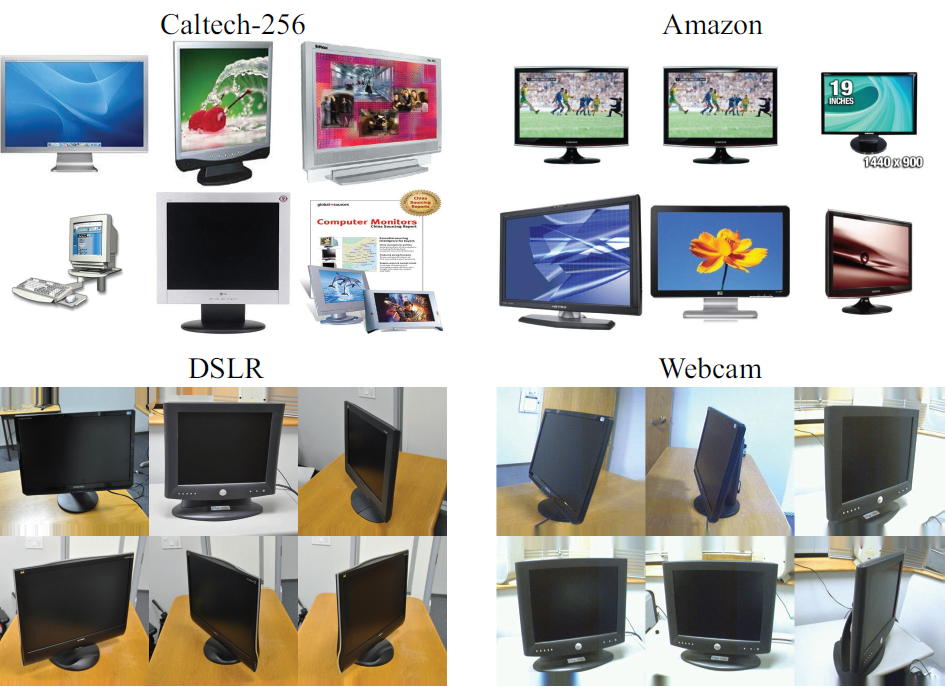
\includegraphics[width=.8\linewidth]{figures/ExampleImages.png}
	\caption[Example from Image Dataset]{Examples Images from the four Image Datasets Caltech10, Amazon, DSLR, Webcam. \cite{Gong.}}
	\label{FigExampleImages}
\end{figure}
\section{Study Procedure and Settings}\label{EmSecStudy}
In this part, the data sampling, parameters and the used kernels are introduced.
Every transfer learning method, which is used in the study is already introduced in chapter \ref{Tl}.
Note that for a fair comparison the heterogeneous methods are not included in the study because they solve a different problem from the \acs{PCTKVM}, which is described above in section \ref{TlSecHetero}.
The basic task in this study is classification with data from the same feature space.\\
The \ac{SVM} and the \acl{PCVM} are the baseline classifier in this study.
The \acs{PCVM} is described in section\ref{Pc}.\\

\subsection{Data Sampling}\label{EmSubSecDataS}
The samples for testing the classifiers are drawn with five times two-fold cross-validation manner.
However, to obtain the differences from training- to test-set and the resulting transfer learning attributes, a sample is not drawn from the dataset as one, but rather obtaining the different domains and draw from one only for training or testing.
This means for example, two image sets \textit{amazon} and \textit{webcam} are not merged together.
Furthermore, the comparability of this study with another study would be lost.
The training set is sampled from \textit{amazon} and the test is from \textit{webcam}.
This is a suggested standard method for cross-validation in transfer learning.\cite{Gong.}
Besides, the datasets are normalised via z-scored.
This can be obtained from equation \ref{EqZTrans} in section \ref{InSubSecTheta}.
\subsection{Kernel}\label{EmSubSecKernel}
A kernel in this work is a symmetric matrix, in the following $\mathbf{K}$, which has to be positive semi-definite and therefore satisfying the Mercer conditions and integrates a similarity (dissimilarity) measure.
It is a inner product of $N$ training pattens, represented as vectors, which is a $N \times N$ matrix:
\begin{equation}
	\mathbf{K}(\mathbf{x},\mathbf{x'}) = \phi(\mathbf{x})^T\phi(\mathbf{x'})
\end{equation}
With $\phi(\cdot)$ as explicit feature mapping function.
Because of its symmetry $\mathbf{K}(\mathbf{x},\mathbf{x'})=\mathbf{K}(\mathbf{x'},\mathbf{x})$.
In its simplest form, the linear kernel, the function becomes $\phi(\mathbf{x}) = \mathbf{x}$ which results in the simple vector dot product $\mathbf{x}\mathbf{x}^T$ as similarity measure. There are various kernels and techniques to construct it. For example, if one replaces the inner product with some metric, e.\,g. Euclidean distance, then the kernel functions are refereed as basis- instead of feature mapping functions.\cite[p. 291-296, 329]{Bishop.2009}\\
In this study almost all kernel machines are using a modified version of the \ac{RBF}- or Gaussian-Kernel.
The 'well known' kernel can be obtained from \cite[p. 17]{Vert.2004} and has the form:
\begin{equation}\label{EqRBFOriginalKernel}
	k(\mathbf{x},\mathbf{x}') = \frac{d(\mathbf{x},\mathbf{x}')^2}{2\sigma^2}
\end{equation}
Where $d$ is the Euclidean distance and sigma is the width of the Gaussian kernel.\\
The used one is suggested from \cite{Duan.2012} and 'replaces' the $\sigma$ parameter with $\frac{1}{A}$ and $A$ as median over the samples: 
\begin{equation}\label{EqRBFAKernel}
	k(x,x') = \exp(-\frac{1}{A}\abs{x-x'}^2)
\end{equation} 
Note $\gamma = \frac{1}{A}$ is a used abbreviation in \cite{Long.2015}.
There are two classifiers with different kernels.
First, the \acs{GFK} uses the implementation of an own supervised $k$ nearest neighbour approach which can be obtained from the website of the author \ref{TlSubSecHomoSymFeature}.
Second, the \acs{PCVM}, because in the cross-validation state for the parameter determination the performance drops dramatically with the use of \eqref{EqRBFAKernel}.
Therefore the \acs{PCVM} uses the proposed \acs{RBF}-Kernel from \cite{Chen.2009}. 
\begin{equation}\label{RBFKernelPCVM}
k(x,x') = \exp(-\frac{\abs{x-x'}^2}{\sigma^2})
\end{equation}
The rest is trained with the suggested one from \eqref{EqRBFAKernel}, although they are used to train with \eqref{EqRBFAKernel}, which is obtained by the source code from the methods.
However, the \acs{TKL} approaches are using it initially.
This is done to compare the pure transfer performance, as independent as possible.

\subsection{Parameters}
The cost Parameter $C$ of the \acs{SVM}, which controls the trade-off between margin and the ability to adapt the decision boundary to points near to it, is set to 10. \cite[p. 421-422]{TrevorHastie.2009}
Finally, the LibSVM implementation which can work with pre-calculated kernels is used. The kernel is described above in section\ref{EmSubSecKernel}.\\
The PCVM as baseline Classifiers has only one parameter $\theta$, which is set to 1 for both sets.
Furthermore, \textit{niter} is set to 600 because we observed that the \acs{pcvm} often terminates somewhere between 500-600 iterations. The threshold is set to 0.001.\\
The parameters for the transfer learning methods are partly obtained from the corresponding papers or with cross-validation. 
The \acs{PCTKVM} and \acs{TKL} algorithms are mainly using the eigenvalue dumping factor $\xi$ which is set to two for the text datasets and 1.1 for the image datasets.\cite{Long.2015}
Furthermore, the \acs{PCTKVM} uses the new kernel with $\gamma=\frac{\sigma}{A}$ in \eqref{EqRBFAKernel}.
Because of that, there is another parameter $\sigma$ which is set to two for the text sets and one for the image datasets.
When it comes to the sigma estimation for \acs{PCTKVM}\textsubscript{$\theta$Est} described in section \ref{InSubSecTheta} the $\sigma$ value is determined for every dataset respectively.
The estimated sigmas are summarized in table \ref{TableThetaEst}. \\
\acs{JDA} has two Model parameters.
First the number of subspace bases $k$, which is set to 100 and the regularisation parameter $\lambda $ which is set to one for both.\cite{Long.}\\
For the \acs{GFK} solution the parameter, number of subspace dimensions are evaluated with cross-validation from $k=\{1,5,10,20,...,100,200\}$ and finally set for the text sets to 40 and to 50 for the image sets.\\
The \acs{TCA} has also one parameter which gives the subspace dimensions and are determined from $\mu=\{1,5,10,20,...,100,200\}$ and is set to $\mu=50$ for both datasets.\\
The goal of the parameter determination procedure was to identify the best performance concerning the parameters.
\begin{table}[]
	\centering
		\begin{tabular}{|c|c||c|c|}
			\hline
			Dataset         & Theta & Dataset & Theta \\ \hline
			Org vs People   & 1.415 & C vs D  & 2.187 \\ \hline
			Org vs Place    & 2.224 & A vs W  & 2.152\\ \hline
			People vs Place & 2.187 & A vs D  & 2.166\\ \hline
			C vs A          & 2.224 & D vs W  & 2.163 \\ \hline
			C vs W          & 2.187 
	\end{tabular}
	\caption{List of the Estimated Thetas of the Text and Image Datasets\label{TableThetaEst}}
\end{table}

\section{Performance Metrics}\label{EmSubSecPerMet}
The Performance of the transfer learning classifier has to be determined and should be compared with others.
There are several metrics which can be used to measure the performance of a classifier.\\
However, before these are defined, there are some basic definitions to make, which are applied to the metrics in the following sections.
These definitions are helping to get an idea of the location- and distribution characteristics of the sample.\cite[p. 216-217]{Teschl.2014}
First, the mean which gives the average value of samples. 
\begin{equation}\label{EqMean}
	\mean{x} = \frac{1}{N}\sum_{i=1}^{N}x_i
\end{equation}
This samples can be for example one of the key figures of one classifier for the 18 datasets. 
The standard deviation is formulated to measure how the samples are distributed around the mean.
\begin{equation}\label{EqStandardDeviation}
s^2=\sqrt{\frac{1}{N-1}\sum_{i=1}^{N}(x_i-\mean{x})}
\end{equation}
In both \eqref{EqMean} and \eqref{EqStandardDeviation}, $N$ is the number of samples. \\
The null hypothesis in this context has the assumption that two classifiers are equal.
If not this hypothesis is rejected.\cite{Alpaydm.1999} 
To determine if the null hypothesis can be rejected, is the goal of the statistics from \ref{EmSubSecResOneDa} and \ref{EmSubSecResMulDa}.
However, before this decision can be made, the performance of an algorithm has to be captured.
In this thesis are four key figures used.
For clarity, the key figures are represented in the result table in percent.
This differs from the origin calculation presented here.
The selection of the key figures are influenced by \cite{Chen.2009}.\\
\subsection{Area under a ROC Curve}
The first metric is the \ac{AUC} which measures exactly what the name says.\cite[p. 13]{Fawcett.}\\
A \ac{ROC} Curve is a technique for visualising and organising classifiers based on their performance.
This curve sometimes also called graph is a two-dimensional plot of the true positive rate on the Y axis and the false positive rate on the X-axis.
It illustrates the trade-off between the benefits and costs.
The more the graph heads north west, the better is the classifier.
Note that if a classifier has a low \ac{ROC} curve near the X axis, then it may be conservative in making an assignment to a positive class because it makes it only with strong evidence.
That means it makes few false positive errors, but they often have a low true positive rate.\cite[p. 4]{Fawcett.}\\
In this thesis, when it comes to two classes, it is interpreted as a lower performance, because the true positive points have a higher probability to be wrongly classified concerning the
negative label.\\
Because the \ac{AUC} is an area in a unit square, it has a value between zero and one.
The statistical interpretation is as follows: "The \acs{AUC} of a classifier is equivalent to the probability that the classifier will rank a randomly chosen positive instance higher than a randomly chosen negative instance."\cite[p. 13-16]{Fawcett.} \\
Concerning a two-class problem, the \acs{AUC} tells us the probability for a member of the positive class and the negative class that the positive one is correctly classified to the positive class and the other respectively. 
For this thesis the build-in Matlab function \textit{[X,Y,~,AUC] = perfcurve(LABELS,SCORES,POSCLASS)} is used.
The function needs the ground truth 'LABELS' and the probabilistic estimate that this point actual belongs to the positive class ('SCORES') determined by a classifier.
With 'POSCLASS' the positive class is specified. In this thesis, '1' is always the positive class.
It gives the arrays X and Y back to create the ROC curve as Matlab plot.
The function output 'AUC' is the needed value for comparison.
Note that with this definition of \acs{AUC}, it makes only sense for two class problems.
For the multi-class problems, the accuracy is more insightful, but the \acs{AUC} is calculated for completeness with '1' as positive label and the rest of the labels as negative.\\
\subsection{Accuracy and Error}
The accuracy is another used metric with:\cite{Long.2015}
\begin{equation}
	Accuracy = \frac{| x : x \in \mathcal{X} \wedge f(x) = y(x)|}{|x : x \in \mathcal{X}|}
\end{equation}
With $f(x)$ as the given label from the classifier and $y(x)$ as the ground truth label.
In other words, how many of the test points are getting the correct labels from a classifier assigned concerning all points.\\
Another way to interpret the accuracy is that it is the relation of the true positive rate and true negative rate to all samples.
The accuracy goes from zero to one because it is normalised.\cite[p. 3]{Fawcett.}
In this thesis, the metric \ac{ERR} is simply calculated with  $Error = 1 - Accuracy$.\\
\subsection{Root Mean Squared Error}
The last metric is the \ac{RMSE}. It takes the root of the squared mean errors.
\begin{equation}
	RMSE = \sqrt{\frac{1}{N} \sum_{i=1}^{n}e_i^2}
\end{equation}
With $N$ as the number of errors which relies on the number of datasets. The  \ac{RMSE} assumes that the errors are normal distributed and unbiased.
It is per definition always higher than the simply \ac{MAE}.
With that, the \acs{RMSE} tends to become increasingly larger in comparison with the \acs{MAE}, as the distribution of the error magnitude becomes larger. 
The \acs{RMSE} penalises the variance of errors by weighting larger absolute errors more than smaller ones.
Note that the \acs{RMSE} is sensitive to outliers.
This key figure is another idea trying to describe the error distribution. \cite{Chai.2014}
\FloatBarrier
\section{Descriptive Statistics}\label{EmSecTest}
In this section, the general performance of the classifiers is shown.
As part of the descriptive statistics, the mean and the standard deviation are used.\cite{Igual.2017}\\
With that, the different key figures over the datasets are summarised.
The performance, in general, is divided into datasets. The full result can be considered in appendix \ref{appaB}.

\subsection{Metric Results}\label{EmSubSecMetricResult}
In this subsection, the performance over the metrics, which are descried earlier, is shown.
The results are summarized in table \ref{TableDescriptiveStatistics}. 
Note that this is data is produced on the fly in the 5x2 cv F test. Therefore the shown results are the mean over ten repetitions of cross-validation.
The standard deviation is shown in brackets. 
The results are split up in the two dataset categories Image and Reuters, respectively.
Furthermore the four metrics error, \acs{RMSE} and \acs{AUC} are applied.
The \ac{ACC} can simply be determined with the error.
The classifier, which is created in the course of this work are italics.
The performance of the best classifier is bold.
The \acs{GFK} implementation supports no probabilistic output and therefore has no \acs{AUC} value in general.
Not that through the cross-validation of the 18 datasets, the means metrics are combined from 180 performance results.\\
It can be observed that the \acs{TKL} with the \acs{SVM} has the overall best performance. 
In general and according to section \ref{TlSecNeg}, it can be seen that negative transfer happens between the baseline \acs{SVM} and the transfer solutions.
But we can note that the \acs{PCTKVM}  \textit{overall outperforms} the \acs{PCVM} in this test.\\
The \acs{SVM} is still better in the image category than the transfer \acs{PCVM}'s. 
This might comes from the fact that the latter has some datasets, where the performance drops dramatically.
Referring to table \ref{BTableFTErr} in appendix \ref{appaB}, we can observe that if the dataset \textit{dslr} and \textit{webcam} are involved, then the performance drop happens. 
We assume that this happens because the datasets are very small, with 295 and 157 samples respectively, because we can rather obtain a good performance on the larger text datasets and usually the larger image datasets in comparison with the \acs{SVM}.
This assumption may be more valid when one takes a look at the comparison, which involves the whole dataset, which is shown in table \ref{BTableCompleteErr}.
Therefore it seems that the \acs{SVM} can handle very small datasets better than the \acs{PCVM} in general. However, again referring to the detailed test results, it states that the \acs{PCTKVM} is often the second best classifier.\\
Additional, we can see that the \acs{SVM} baseliner has an overall better performance than the \acs{PCVM} baseliner.
Apart from the size of datasets, it might be that because of the differences in the distribution caused by the dataset; it might be a better idea for transfer learning to find a hyperplane, which separates the classes best, rather than modelling it via probabilistic.
In fact, the performance is of the \acs{TKL} is always better than the performance of \acs{PCTKVM}.\\
Furthermore we can observe that the \acs{PCTKVM}\textsubscript{$\theta$Est} is in general worse than the \acs{PCTKVM}. 
Because these two approaches only differ in the $\theta$ value, we can say that the $\theta$ estimation approach described in section \ref{InSubSecTheta}, works out not very well.
In fact, the estimation was originally designed for regression and classification \cite{Kitayama.2011}. However, it seems that the value of the estimation is too 'smooth' and the probabilistic estimation for one class are 'overlapping' in the other classes space.
This space, would one intuitively assign to the other label.
This might be similar to the problem of the \acs{RVM} from \cite{Chen.2009}, Where it assigns a negative weight in the heart of the positive class.\\
The essence of the standard deviation in table \ref{TableDescriptiveStatistics} states the overall performance range in the datasets, which fluctuates with respect to the composition of the datasets.
Therefore, to make a valid assumption on the standard deviation concerning the classifiers, we again have to look in the detailed result table \ref{BTableFTErr}.
As pointed out in the results of Chen et al. in \cite{Chen.2009} and with our results again, the range of standard deviation for the \acs{PCVM} is not that kind of a problem. 
However, when it comes to the \acs{PCTKVM}\textsubscript{$\theta$Est}, we see that the range of standard deviation, especially for the text datasets, is higher in comparison with the deviation of the remaining classifiers.
Since \acs{PCTKVM} and \acs{PCTKVM}\textsubscript{$\theta$Est} only differ in the theta value, we can say that the fluctuation of performance in this test also depends on the theta.
The fact that all \acs{PCVM}'s are random initialised is not critical because we can observe that the standard deviation are not greatly higher in comparison with the other classifiers form table \ref{BTableFTErr}. 
\begin{table}[]
	\centering
	\resizebox{\textwidth}{!}{%

	\begin{tabular}{@{}lccllcccc@{}}
		\toprule
		ERR     & SVM   & PCVM  & PCTKVM\textsubscript{$\theta$Est} & PCTKVM & TCA   & JDA   & GFK   & TKL              \\ \midrule
		Reuters & 31.82(2.02) & 34.19(3.65) & \textit{30.03}(6.63)    & \textit{26.12}(2.97)  & 30.87(3.24) & 32.95(2.54) & 34.53(2.74) & \textbf{22.70}(2.17) \\
		Image   & 61.51 (2.75)& 68.13(3.11) & \textit{63.53} (3.48)   & \textit{62.64} (3.35) & 59.56(3.33) & 59.39(3.32) & 64.24(2.96) & \textbf{58.25}(7.63) \\\midrule
		RMSE    & SVM   & PCVM  & PCTKVM\textsubscript{$\theta$Est} & PCTKVM & TCA   & JDA   & GFK   & TKL              \\
		Reuters & 31.88 (8.43) & 34.48(5.93) & \textit{30.77} (10.35)  & \textit{26.28} (9.32) & 31.03(9.00) & 33.05(8.81) & 34.63(6.28) & \textbf{22.81}(7.63) \\
		Image   & 61.59(14.71) & 68.23(6.88) & \textit{63.64} (9.15)   & \textit{62.76}(9.35)  & 59.67(14.76) & 59.50(14.81) & 64.33(15.39) & \textbf{58.36}(13.63) \\\midrule
		AUC     & SVM   & PCVM  & PCTKVM\textsubscript{$\theta$Est} & PCTKVM & TCA   & JDA   & GFK   & TKL              \\
		Reuters & 69.00 (2.33) & 70.96(3.99) & \textit{76.47} (8.63) & \textit{79.36}(4.82)  & 72.32(3.78) & 69.11 (3.13) & -     & \textbf{83.46} (2.26)\\ \bottomrule
	\end{tabular}}
	\caption[Result of Cross-Validation]{The results of the transfer learning classifiers with cross-validation under the four metrics on the 18 datasets.\label{TableDescriptiveStatistics}}
\end{table}
\FloatBarrier
\subsection{Time Results}\label{EmSubSecTimeResults}
The next comparison is over the mean computational time, which a classifier needed to train and test the datasets.
The baseline takes part in the time measure for the transfer learning solution, because it is about to test for example if the \acs{SVM} can handle the subspaces or a different kernel in proper time.
Note that that the computational time is summarised in ranks.
The first rank is assigned for the fastest and the last for the slowest.
Average ranks are assigned for ties with respect to ranks.
With this, there are the means of the datasets combined, and the ranks are the result of it.
The table \ref{TableMeanTimeRank} shows the mean of these ranks.
The second row of the table shows the mean time over all 18 datasets in seconds.\\
The result of the time ranking is unambiguous, with the \acs{SVM} as the fastest classifier. 
However, this is no surprise, because it is beside the \acs{PCVM} the baseline classifier, and has because of this the lowest computational complexity, which results in lower training and testing time.
Obviously, because the other solution are trying to do the transfer learning, which results in higher complexity.\\
Although the complexity of \acs{PCVM} and \acs{SVM} are comparable, in practice, more precisely, datasets with two domains, we observed that the $\theta$ optimisation takes forever.
It seems that in the transfer learning setting, the local optimum for the next theta is hard to obtain.
Another point to mention is that the \acs{PCVM} does not converge very well and uses the full 500 iterations. 
This, combined with the $\theta$ optimisation in every iteration, leads to the high computational time.\\
Although the ranks from \acs{PCTKVM}\textsubscript{$\theta$Est} and \acs{PCTKVM} are bad in comparison with the other classifiers, we have, by integration of the new kernel, greatly improved the speed.
This has two reasons: 
The first is that the $\theta$ optimisation is replaced with a fixed value or the estimation.
The second is that the new \acs{PCVM}'s are converge much faster and therefore may need fewer iterations to finish.
The theta estimation in comparison with the fixed value makes a mean difference from 11.52 seconds.\\
The computer which is used to determining the needed time was an Acer Aspire V5-573G, containing an Intel Core i5 4200U Prozessor with 2x 1.60 GHz, 8GB of main memory and a NVIDIA GeForce GT 750M with 4GB of memory as graphic card.
\begin{table}[h]
	\centering
	\resizebox{\textwidth}{!}{%
			\begin{tabular}{@{}cccccccccc@{}}
				\toprule
				Time & SVM  & PCVM &  PCTKVM\textsubscript{$\theta$Est} & PCTKVM & TCA  & JDA  & GFK    & TKL  \\ \midrule
				Rank & \textbf{1.08} & 8.00  & \textit{4.46 }& \textit{5.46}  & 4.10 & 5.23 & 4.96 & 2.71\\
				Sec & \textbf{3.99} & 353.75  & \textit{17.56} & \textit{17.19}  & 5.88  &6.70 & 12.52 & 4.40 \\ \bottomrule
			\end{tabular}}
	\caption[Comparison of Mean Computational Time]{The mean computational time rank of the classifiers.\label{TableMeanTimeRank}}
\end{table}

\subsection{Number of Support Vectors}\label{EmSubSecNumberSV}
The number of support vectors are an indicator of the complexity of a model. 
Note that although we defined for the \acs{RVM} and \acs{PCVM}, that the model vectors are relevance vectors, we will stick to support vectors in general just for simplicity.\\
May many support vectors are leading to a low training error rate, but with the growing complexity, there may be more test errors. 
This happens because of the bad generalisation abilities of the model.\cite[p. 81]{Igual.2017}\\
Another explanation for a large number of support vectors is that the dataset is complicated. For example, the dataset tends to be inseparable.\cite[p. 78;86]{Abe.2010}
However, in testing the transfer learning algorithms on the specific dataset may a different view arises. 
Thus the model complexity is large for the transfer learning methods with the as \acs{SVM} classifier, the classification performance is not that bad in comparison with the sparse \acs{PCTKVM} or \acs{PCVM}, referring to table \ref{TableDescriptiveStatistics}, \ref{TableFiveTwo} and \ref{TableFriedman}.
However, we want to point out that in general, lesser support vectors in a model leads to more compact models.\cite[p. 349]{Bishop.2009}\\
This is the strength of the \acs{PCTKVM}\textsubscript{$\theta$Est} and \acs{PCTKVM}, although the sparse model of the \acs{PCVM} has a worse performance, our solutions are obtaining relative sparse model by maintaining a competitive performance on difficult datasets.
The mean number of support vectors needed by a classifier is split up dataset categories and is summarised in table \ref{TableMeanNSV}. 
The mean number of the datasets are shown on the left-hand side of the name in brackets.
\begin{table}[h]
	\centering
	\resizebox{\textwidth}{!}{%

		\begin{tabular}{@{}ccccccccc@{}}
			\toprule
			N. SV.  & SVM    & PCVM  &  PCTKVM\textsubscript{$\theta$Est} & PCTKVM & TCA   & JDA    & TKL  \\ \toprule
			Reuters(1153.66) & 482.35 & 46.93 &   \textbf{3.02}          &    \textbf{3.02}   & 182.70 & 220.28  & 190.73                                                 \\
			Image(633.25)   & 309.90  & 68.40 &    \textbf{ 50.02 }      &   \textit{54.88} & 253.30 & 287.433  & 382.53                                          \\ \bottomrule
		\end{tabular}
	\caption[Comparison of Number of Support Vectors]{The mean of number support vectors of a classifier for Reuters and Image datasets.\label{TableMeanNSV}}}
\end{table}
\FloatBarrier
\section{Comparison over one Dataset}\label{EmSecOneData}
The 5x2 cv F test is a statistical tool to compare the performance of supervised classification learning algorithms on one dataset. \cite{Chen.2009}
The first approach, the 5x2 t-test, was designed by Dietterich in 1998. \cite{Dietterich.1998}
The improved 5x2 cv F test should have less Type I error (wrongly reject null hypothesis) and a higher power (probability of detecting a difference if it exists) than the proper.\cite{Alpaydm.1999}
It is in general designed to compare two classifiers.
As mentioned in \ref{EmSubSecDataS} the sample is drawn with the use of the cross-validation approach and randomly splits up the data in 2 parts, fold one and fold two.
This is repeated five times. 
To determine whether a classifier is indeed better than another, the test statistic has to be calculated.\\
Suppose that $p_i^{(j)}$ is the difference between the error rates of two classifiers on fold $j = 1,2$ and replication $i=1,..5$.
The average of a replication is $\mean{p_i} = (p_i^{(1)}+p_i^{(2)})/2$.
And the estimated variance is $s_i^2=(p_i^{(1)}-\mean{p_i})^2+(p_i^{(2)}-\mean{p_i})^2$.
Then the value to determine statistical significance in the differences of the errors is calculated as:
\begin{equation}
	f = \frac{\sum_{i=1}^{5}\sum_{j=1}^{2}(p_i^{(i)})^2}{2\sum_{i=1}^{5}s_i^2}
\end{equation}
This value is approximately F distributed. It has ten and five degrees of freedom.
The null hypothesis that the classifiers have the same error rate is rejected with a confidence of 0.95 if the f is greater than 4.74. \\
An Idea of the F distribution can be obtained from \cite[p. 338-340]{Teschl.2014}
Critical values from this distribution can be obtained from a statistic table, e.\,g. \cite[p. 591]{Bortz.2010}.
Note that this explanation focuses only on the error metric.
However, it should be possible to do this test with other metrics as well.\\
This is possible because the idea of this statistic is to determine if the metrics, e.\,g. error, of two classifiers, are drawn from the same distribution (null hypothesis).\cite{Alpaydm.1999}

\subsection{Result and discussion}\label{EmSubSecResOneDa}
The result of the 5x2 cv F test is shown in table \ref{TableFiveTwo}.
In this table the cells are not showing the value of error in percent, but rather the summary of the wins,  loses and ties against the \acs{PCTKVM} as competitor algorithm.
The row Significant is showing the amount of the significant wins loses or ties of the total.
Note that because of this setup, one has to read the table the other way around. 
A lose for a classifier shown in this table is a win for the \acs{PCTKVM} and vice versa. 
A win is determined by comparing the performance of the two folds (10 runs).
If there are more wins out of the 10 for one classifier, then it is a win for it. If the wins and losses are equal, then is a tie. 
That means a tie does not represent a real equal performance, but rather that the wins and losses are even.\\
With the descriptive statistic table from \ref{TableDescriptiveStatistics}, we can not make a valid statistical evidence if the difference of performance is significant, i.\,g. we can reject the null hypothesis.\cite[p. 9]{JanezDemsar.2006}
We can only observe trends and assume significance.\\
The results are showing, that the \acs{PCTKVM} does a decent job in the Reuters dataset.
In fact, it wins every time against the baseliners and the transfer learning solutions, except against the \acs{TKL}, partly even significant.\\
The \acs{PCTKVM} can outperform the baseline \acs{PCVM} four times significant out of 6 wins with the text dataset.
The performance gap is not that large at images, but sill our approach wins every time out of twelve datasets with one significant win.\\
Compared to the \acs{PCTKVM}\textsubscript{$\theta$Est}, it wins five out of 6 times with one significant and one tie. 
When it comes to image dataset the performance, between the two, is more balanced.
We assume that this could have two reasons:
One might argue that the $\theta$ for the image is not well selected, but it is selected with a cross-validation process to determine the best performance. Another reason could be that the $\theta$ estimation does a better job when it comes to images or takes values that are not considered in the parameter determination.\\
Considering the performance with the image dataset with respect to the remaining classifiers, the baseline \acs{SVM} can win six times against the \acs{PCTKVM}, with one significant, while the latter only wins four times.
The same 'worse' result happens with the transfer learning classifiers, with a similar result.
As already discussed in section \ref{EmSubSecMetricResult}, a reason for this might be the small datasets.
Note that this statistic has ten and five degrees of freedom.
\begin{table}[]
	\centering
	\resizebox{\textwidth}{!}{%
	\begin{tabular}{@{}cccccclc@{}}
		\toprule
		Win-Lose-Tie & SVM    & PCVM  & PCTKVM\textsubscript{$\theta$Est}   & TCA   & JDA   & GFK    & TKL    \\ \midrule
		Reuters         & 0-6-0 & 0-6-0  &\textit{4-1-1 }&0-6-0 & 0-6-0 & 0-6-0 & 6-0-0  \\
		Significant  & 0-3-0 & 0-4-0  & \textit{0-0-0} & 0-2-0 & 0-3-0 & 0-4-0  & 0-0-0   \\ \bottomrule
		Image         & 6-4-2 & 0-12-0 &\textit{ 4-3-5} & 9-3-0 & 6-3-3 & 6-6-0 & 10-1-1\\
		Significant  & 1-0-0  & 0-1-0  & \textit{1-0-0 }& 2-1-0 & 3-0-0 & 2-0-0  & 4-0-0   \\ \bottomrule
	\end{tabular}}
	\caption[Result of the 5 x 2 cv F Test]{The result of the 5 x 2 cv F test to compare classifiers on one dataset under the Error metrics. The competitor is PCTKVM, and the result is shown as the number of wins, losses and ties.\label{TableFiveTwo}}
\end{table}
\FloatBarrier
\section{Comparison over multiple Datasets}\label{EmSecMulDa}
Testing algorithm over only one dataset has a certain risk. The problem is with a high amount of tests like it is done in \ref{EmSecOneData} is that a certain proportion of the null hypotheses are rejected due to random chance. This issue is a well known statistical problem. The goal is to control the family-wise error: The probability of making in any of the comparisons at least one Type 1 error.
The Friedman test is used as a statistic to compare supervised classification learning algorithms over multiple Datasets.
It is first introduced, as the name says, by Friedman in 1937. It is a non-parametric equivalent of the repeated-measures of \ac{ANOVA}.\cite[p. 9-10]{JanezDemsar.2006}\\ 
\subsection{Analysis of Variance}
The ANOVA, briefly, compares the variability between the classifiers, variability between datasets and the remaining error variability. 
Is the between classifier variability is significantly larger than the error variability, the null hypothesis can be rejected with the conclusion that there are differences between the classifier.
\acs{ANOVA} makes some assumption that cannot be held for the comparison of classifiers and therefore the Friedman test is chosen.
For example, \acs{ANOVA} has the assumption of sphericity, and this is not guaranteed for comparison of multiple classifier and datasets.\cite[p. 10]{JanezDemsar.2006}\\
Sphericity is the condition that the difference between samples is homogenate. If not the \acs{ANOVA} F value will be too large.\cite[p. 152]{Hinton.2004}

\subsection{Friedman Test}
The Friedman test ranks the classifiers for each data separately. The best one has rank 1, the second has rank 2 and so on.
The average rank is assigned in case of a tie. For $r_i^j$ as the $j$-th rank of $k$ algorithm on the $i$-th of $N$ datasets.
And with $R_j = \frac{1}{N}\sum_{i=1}^{N}r_i^j$ as the average rank of an algorithm, the Friedman tests compares the average ranks.
The null hypothesis has the assumption that all classifiers are equal and hence the average ranks $Rj$ should be equal.
In equation \eqref{EqFriemanXF} the formula for the F value is shown.
\begin{equation}\label{EqFriemanXF}
	\mathcal{X}_F^2 = \frac{12N}{k(k+1)}\Bigg[\sum_{j=1}^{k}R_j^2 - \frac{k(k+1)^2}{4} \Bigg]
\end{equation}
It is distributed according to $X_F^2$ (Chi-Square-Distribution).
This distribution has $k-1$ degrees of freedom. However, this takes only place if $N$ and $k$ are high enough.
A solid numbers would be $N>10$ and $k>5$. \cite[p. 11]{JanezDemsar.2006}\\ We are about the 'solid' numbers with eight classifiers and 15 datasets.
However, Iman and Davenport showed in \cite{RonaldL.Iman.} that the Friedman $\mathcal{X}_F^2$ value is needless conservative and proposed a better statistic which is shown in equation \eqref{EqImanFriedman}.\cite[p. 11]{JanezDemsar.2006}
\begin{equation}\label{EqImanFriedman}
	F_f= \frac{(N-1)\mathcal{X}_F^2}{N(k-1)-\mathcal{X}_F^2}
\end{equation}
This is statistic is F distributed with $k-1$ and $(k-1)(N-1)$ degrees of freedom.\\
The Friedman test only determines is there any significant difference at all. 
If the null hypothesis can be rejected (Significant difference), we can proceed with the post-hoc test to determine which classifiers are significantly different.
Significance exists, if the F value from \eqref{EqImanFriedman} is equal or above the critical values, for a confidence level of 0.95, from the F distribution.\cite[p.11]{JanezDemsar.2006}\\
In this article, the Bonferroni-Dunn test is used for the post-hoc test as it is used in \cite{Chen.2009}.
Finally, we can reject the null hypothesis and proceed with the post-hoc test.
The performance of two algorithms is significantly different if their average ranks differ by at least the critical difference. 
This difference needs the parameter $q_\alpha$ and is set to 2.690, because of eight classifiers and the confidence level of $\alpha = 0.5$.
So the confidence levels of Friedman and 5x2 cv F test are the same.
The critical difference is shown in equation \eqref{EqCriticalDifference}.\cite[p. 11-12]{JanezDemsar.2006}
\begin{equation}\label{EqCriticalDifference}
	CD = q_\alpha\sqrt{\frac{k(k+1)}{6N}}
\end{equation}
Note that the Friedman test and the post-hoc test is implemented on our own, because it seems that Matlab\footnote{https://de.mathworks.com/help/stats/friedman.html} provides only the first part of the test (Original Friedman), which is the Friedman test without the described improvements from Iman and Davenport.

\subsection{Result and Discussion}\label{EmSubSecResMulDa}
The in the following discussed results are covering the 18 datasets.
The result of the Friedman test is separated into two tables.
The first \ref{TableMeanRank} is showing the mean ranks under the performance metrics.
This is done by ranking the mean of the performance according to one dataset and results in 18 ranks per classifier. A tie is assigned if the mean of two classifiers are equal.\\
The second \ref{TableFriedman} shows the Friedman test result and the corresponding post hoc test. 
It shows the results of Friedman test with the corresponding post hoc test. The critical difference is computed according to equation \eqref{EqCriticalDifference}.
The key values are showing the difference of mean ranks against the mean rank of the \acs{PCTKVM}.
To see if a classifier has a significant difference in performance the key value in the table has to be at least the critical difference.
For clarity, it shows not the absolute rank difference, but rather with the corresponding sign.
That means for error, \acs{RMSE} a classifier is better if the rank difference is negative and worse if it is positive.
For \acs{AUC} and \acs{ACC} it is vice versa.
The bold cells are indicating any significance.
Note that one may draw further results out of the results by just taking the mean ranks of two classifiers from table \ref{TableMeanRank}, subtract them and compare the difference against the critical difference. \\
Although we have omitted some metrics in the previous discussion, it seems reasonable to show all four metrics, because they differ more in this test in comparison with the previous statistics.
Finally we can provide a $7\times 119$ degrees of freeman for error, \acs{RMSE} and accuracy and $6\times102$ degrees of freedom for \acs{AUC}.\\
With the results of table \ref{TableFriedman}, we can say that the \acs{PCTKVM} can outperform the \acs{PCVM} significant in three out of four metric categories. The same is valid when it comes to \acs{GFK}.\\
In comparison with the \acs{PCTKVM}\textsubscript{$\theta$Est}, we can say that the \acs{PCTKVM} is in general better but not significant.
In fact the \acs{SVM} is a little bit better than the \acs{PCTKVM}\textsubscript{$\theta$Est} and always better as the \acs{PCVM} in the overall comparison.\\
By comparing \acs{TKL} with the \acs{PCTKVM} we can observe that the first is indeed better, almost but not significant.
The performance of the \acs{PCTKVM} against \acs{JDA} and \acs{GFK} are comparable.
Furthermore, it appears that aligning the conditional probabilistic distributions are no guarantee for a good transfer learning performance concerning \acs{JDA}. However, this is the main extra effort or difference, which is done by \acs{JDA} in comparison with the \acs{TCA} and the \acs{PCTKVM}: Aligning the conditional and marginal probability distribution instead of just aligning the latter.\cite{Long.}\cite{Pan.2011}\cite{Long.2015}\\
Another important fact which arises from the result is that the \acs{SVM} by incorporating the kernel from section \ref{EmSubSecKernel}, very competitive to the transfer learning solutions.
Note that we do not say, that the kernel causes the good performance, but we want to point out the difference to the suggested setting of the LibSVM\footnote{http://www.csie.ntu.edu.tw/\~cjlin/libsvm/faq.htm\#f506}.
Only the \acs{TKL} can significantly outperform the \acs{SVM}.
Furthermore, the differences of \acs{PCTKVM}\textsubscript{$\theta$Est} and the \acs{TKL} are actual significant. 

\begin{table}[]
	\centering
	\resizebox{\textwidth}{!}{%
			\begin{tabular}{@{}lcccccccc@{}}
				\toprule
				Mean Ranks & SVM  & PCVM & PCTKVM\textsubscript\{$\theta$Est\} & PCTKVM & TCA  & JDA  & GFK  & TKL  \\ \midrule
				ERR        & 4.5  & 6.94 & 4.94                                & 3.78   & 3.39 & 4.11 & 6.56 & 1.78 \\
				RMSE       & 4.33 & 6.94 & 4.94                                & 3.89   & 3.39 & 4.22 & 6.5  & 1.78 \\ \midrule
				AUC        & 3.39 & 2.94 & 4.33                                & 4.94   & 3.22 & 4    & -    & 5.17 \\
				ACC        & 4.5  & 2.06 & 4.06                                & 5.22   & 5.61 & 4.89 & 2.44 & 7.22 \\ \bottomrule
			\end{tabular}}
	\caption[Mean Ranks under the Perfomance Metrics]{The Mean Rank of the tested classifiers under the Metrics ERR, AUC, and RMSE.	\label{TableMeanRank}}

\end{table}

\begin{table}[]
	\centering
	\resizebox{\textwidth}{!}{%
	\begin{tabular}{@{}cccccccccc@{}}
			\toprule
			Metrics & Friedman test & CD\textsubscript{0.05} & SVM   & PCVM  & PCTKVM\textsubscript{$\theta$Est} & TCA   & JDA   & GFK   & TKL   \\ \midrule
			ERR     & 0.00          & 2.20                     & 0.72  & \textbf{3.16}  & \textit{1.16}                                & -0.39 & 0.33  & \textbf{2.78 } & -2    \\
			RMSE    & 0.00          & 2.20                     & 0.44  & \textbf{3.05}  & \textit{1.05}                                & -0.5  & 0.33  & \textbf{2.61}  & -2.11 \\ \midrule
			AUC     & 0.01          & 2.20                     & -1.55 & -2    & \textit{-0.61  }                             & -1.72 & -0.94 &-  & 0.23  \\
			ACC     & 0.00          & 2.20                     & -0.72 & \textbf{-3.16} & \textit{-1.16}                               & 0.39  & -0.33 & -\textbf{2.78} & 2     \\ \bottomrule
		\end{tabular}}
	\caption[Result of Friedman Test with Bonferroni-Dun as Post-Hoc Test]{The result of the Friedman Test with Bonferroni-Dunn as Post-Hoc Test to compare classifiers over multiple Datasets.	\label{TableFriedman}}
\end{table}
\FloatBarrier
\section{Conclusion}\label{EmSecConc}
Summarising, the study is made of the three main parts of the statistic. On first sight, it may be strange to compare first the difference between single datasets and proceed with an overall test. This is made because of two analytical reasons. First, the study has two different kinds of datasets (image and text) and many subcategories and subsets. With the single test, it can be determined if there is a significant difference between the performance of classifiers and datasets. When it comes to a real-world scenario, the choice of a classifier may depend on his strengths and weaknesses to solve a task on a corresponding kind of dataset. With this listing of the performance may one can choose more precisely which classifier he chooses for the job. At least for text documents and images.\\
On the other hand from the scientific viewpoint, the comparison over all used datasets and the results in performance giving the most useful insights.\\
Summarizing, we proofed the success of the integration of transfer learning into the \acs{PCVM} by showing significant differences in the performance between these two. Furthermore, our approach can compete with current transfer learning solutions and is just significantly outperformed by one method.\\
We proofed it with an extensive study over 18 dataset compositions of two data categories, which are common in testing of transfer learning, and by finally incorporating two statistical procedures to determine significance.
